\chapter{System Evaluation}\label{chap:eval}
One of the aims stated for this study, as listed in the Chapter~\ref{sec:Introduction}, was to write a Python application with scalability in mind. Therefore, this chapter is devoted to presenting a thousand-feet view of the application so that the implementation described in former chapters could be taken as only one of the many possibilities to realise the intended system characteristics as well as functionality. The second section of the chapter presents a discussion of SmartNotes application metrics gathered using benchmarking tools such as \texttt{autobench} or \texttt{siege} and statistics from the Google App Engine dashboard. The present chapter, together with Chaper~\ref{cha:conclusions}, also summarises the results of the subject of this study. 
 
\section{Presentation of the final result}\label{sec:result}
Apart from a client-server architecture whose segments were presented in Figure~\ref{fig:smartnotes_components}, SmartNotes has the features of flexibility, scalability and security described in Section~\ref{sec:gae}. The web interface of the application is a simple, internationalized one that provides general information about the project and allows the iterated users access its functionality. Currently, the latter involves merely creating a SmatNotes account by using the Google Account as described in Section~\ref{subsec:ismartnotes_activation} and later receiving an activation key, the process being straightforward as presented in Figure~\ref{fig:sn_web_interface}. Finally, the users pass the activation code to the iSmartNotes application in order to take the advantage of synchronization feature allowing the users, as described in Section~\ref{sec:functionality_descr}, to work on their notes and perform synchronization whenever they may wish. The main iSmartNotes window is presented in Figure~\ref{fig:ismartnotes_window}; specifically, it has a simple text area where notes can be edited, and a \texttt{Sync} button that, depending on network connectivity, will perform synchronization on the local machine or additionally using the SmartNotes network infrastructure. This basic attempt realises the functionality, excluding sharing and grouping notes which are extensions to the present functionality and will be added to the SmartNotes application beyond the focus and implementation completed in this study. It can be clearly noted that the tool cannot compete with such applications like the ones introduced in Section~\ref{sec:popular_apps}. Yet, the related work was used as a inspiration for creating a scalable foundation that could be later become more complex by adding additional functionality, hence making the gathered experience further expanded and rendering SmartNotes more attractive to users. Finally, the SmartNotes blog, feedback form and hosting the source code on a well known Open Source service does not only point to gather users’ attention, but also to find developers who find the idea interesting and collaborate on it. 
 
Technologies chosen here provide a well documented and truly active environment with a relatively low access barrier allowing direct involvement in a short time. Some of the chosen solutions, like Django or Mercurial, could become substituted with their equivalents among different language environments or using the Java language as a universal binding for the tools\footnote{Java programming language is wide know for its dynamic curve of development and impressing thread management. These features are few on the list of characteristics motivating the existence of such projects as JRuby, Jython or Quercus which are Java implementations of respectively Ruby, Python and PHP languages. That way, different runtimes can be used in one common environment, taking advantage of all of Java’s features.}.       
\begin{figure}[ht]
  \begin{center}
    \subfigure[\textbf{SmartNotes homepage with basic information and authentication}.]{\label{fig:sm_main}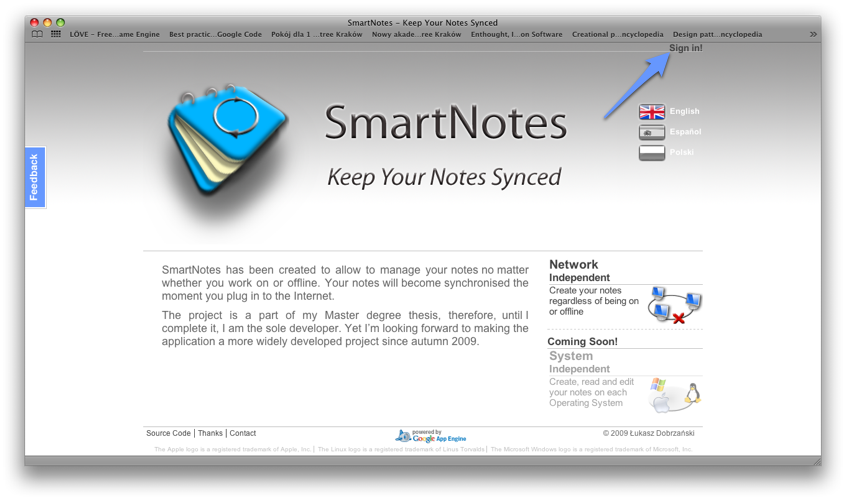
\includegraphics[scale=0.5]{img/SNmain_page.png}}
    \subfigure[\textbf{Authentication using the Google account}.]{\label{fig:sm_signin}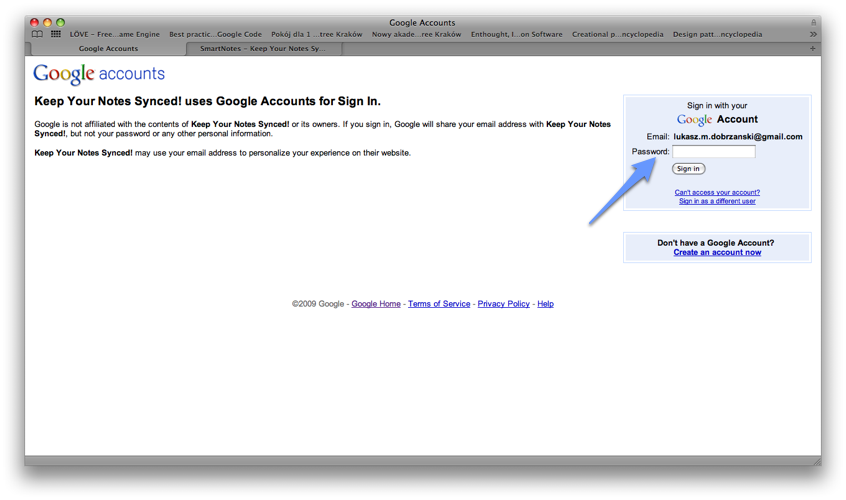
\includegraphics[scale=0.24]{img/SN_signin.png}}
    \subfigure[\textbf{Obtaining the SmartNotes activation key}.]{\label{fig:sm_getSNkey}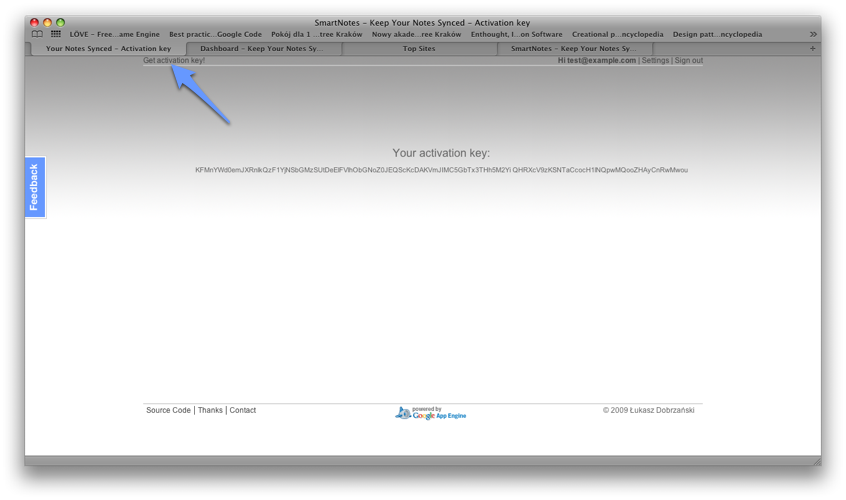
\includegraphics[scale=0.24]{img/SNget_activation_key.png}}
  \end{center}
  \caption{The view on the public web-based SmartNotes interface with basic information regarding the project and authentication.}
  \label{fig:sn_web_interface}
\end{figure}
That direction of development appears to be gathering popularity and is worth attention. However, the chosen set of components including:
 \begin{itemize}
        \item{Google App Engine -- as a platform providing scalable infrastructure and additional useful API's for mailing, imaging or remote task queues.}
        \item{Django famework -- one of Python web frameworks which attracts more and more developers trough its clean architecture, out-of-the-box usability and strong community.}
        \item{Mercurial -- pure Python version control system with a well-designed support for HTTP protocol and a zero cost of administration.}
 \end{itemize} 
is remains significantly powerful, allowing to carry out the desired functionality with easiness for further development, an aspect that should be always recalled during any design process or when choosing between concurrent solutions. That, combined with system streamlining for concrete use cases, determines why the entire system concept is highly desirable when building scalable systems.
        
\begin{figure}[ht]
\begin{center}
\includegraphics[scale=0.5]{img/SN_ismartnotes_window.pdf}
\caption{The view on the iSmartNotes application window.}
\label{fig:ismartnotes_window}
\end{center}
\end{figure}
% gae_best_practises_plus_load_tests
\section{Performance tests}\label{sec:performance}
Performance testing form does strongly depend on the research scope. Testing the application performance is only a general name for the process that should become narrowed to a single parameter or set of well defined properties. The usage of wright tool does also matter just as making appropriate assumptions and choosing wright model used as otherwise measured values could not match the real application characteristics.   

The analyses done in this chapter are fallowing the guidelines as defined in~\cite{gae_best_practises_plus_load_tests} for testing applications that use Google App Engine:
\begin{itemize}
	\item{Use production system. Most of web frameworks provide a development including sever that can be easily run on the local machine. What speedups the development at one side cant be used for production purposes. This environment divers significantly from the deployment system and cant be to give much information of final system performance.}
	\item{Gradual ramp up. The goal of load tests is to probe the system reaction for a certain input parameter sets. Therefore its strongly desirable to make it remind the realistic cases. Besides the resources of Google App Engine are granted only when the application needs them. That motivates a wrap up just before the wright test takes place.}
	\item{Realistic load. Is seams pointless to run test for a situation that the system is unlikely to reach.}
\end{itemize}
The fallowing part of this subsection presents a graphical illustration for selected performance metrics of SmartNotes application running on Google App Engine. Taking into account the parameters such as the rate of opened connections and reached request rate the analyses in the first step will focus on the variations of the response rate and will be finalised with a comparison of the average response time between different techniques. This includes a internalized dynamic content, cached page and same page served as static content. The first is a most classical case when some parts of page depending on state may differ, second one makes use of highly popular caching technique and lastly the special infrastructure devoted only for serving static content. All of these will become wider dissed by analysing corresponding results. 

The view on dashboard of SmartNotes application shown in Figure~\ref{fig:sn_dash_view} exposes a plot of request rate timeline for two different scenarios. The first  one marked as~\textit{(a)} illustrates a regular usage case with none anomalies wheres the second figure~\textit{(b)} presents a case when outgoing bandwidth became exceeded. This is most basic way of tracking the application performance and status. Providing couple of other tools which were discussed in Section~\ref{sec:gae_general} admin interface is truly functional yet easy to use. Providing a logs browser it leaves a place where user can place his application specific informations on several logging levels.     
\begin{figure}[ht]
  \begin{center}
    \subfigure[\textbf{Regular situation with average of about one\newline request per second}.]{\label{fig:dash_normal}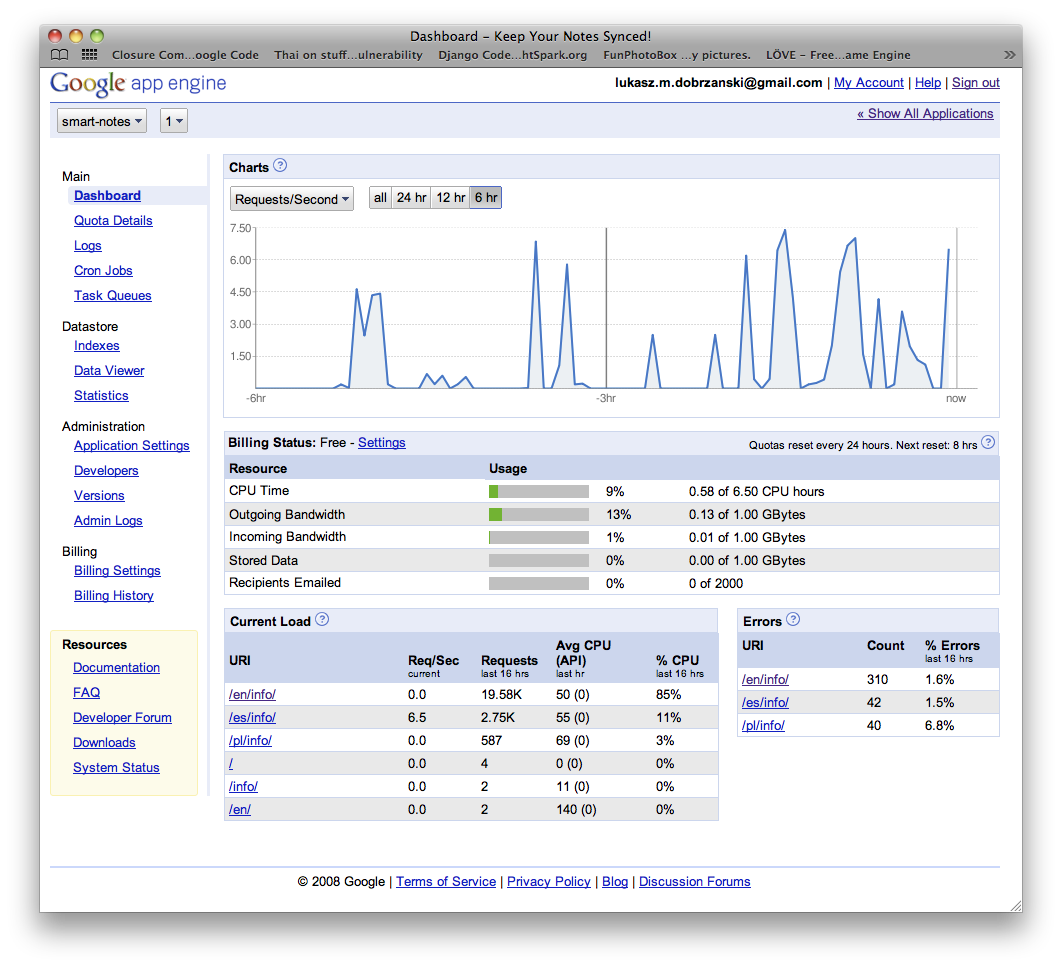
\includegraphics[scale=0.18]{img/DASH_Regular_stats.png}}
    \subfigure[\textbf{Application reaching the outgoing bandwidth limit on heavy traffic situation with the maximum of 170 requests per second}.]{\label{fig:dash_out_of_bandwith}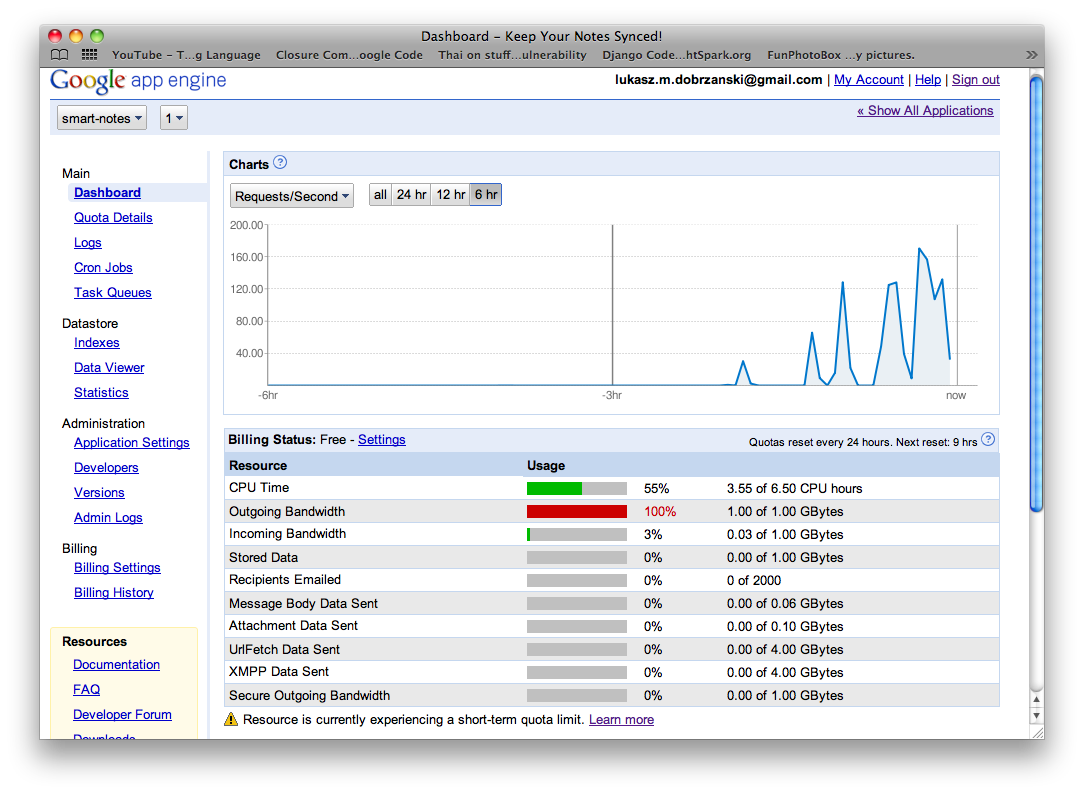
\includegraphics[scale=0.2]{img/DASH_Out_of_bandwith.png}}
  \end{center}
  \caption{The view on the public web-based SmartNotes interface with basic information regarding the project and authentication.}
  \label{fig:sn_dash_view}
\end{figure}
The system of quotas of introduced by Google provides to phase limitations the daily limits and narrowed most common to minute quotas.The second one is a protection for load high peaks or any malicious or testing software that without it could let to letting the target application out of resource in just a couple of minutes. Thats exactly the case uncounted during the tests by receiving responses with \texttt{503 Service Unavailable} status codes when crossing the short tame quota and \texttt{403 Forbidden} responses after running over the daily limits.

The author has chosen Open Source tools like \texttt{httperf} from HP and \texttt{autobench} wrapper to carry out the tests for the main SmartNotes web page. This tools were chosen beyond others researched\footnote{That list includes tools like \texttt{siege} and \texttt{ab} which are popular Open source load testing programs.} due support for a gradual increase of connection rate and extended output. Each of the tests which results are presented in Figures~\ref{fig:sm_benchmark_normal}, \ref{fig:sm_benchmark_cache}, \ref{fig:sm_benchmark_static} and \ref{fig:sm_resp_time_comapre} uses the same set of input parameters:
\begin{itemize}
	\item{500 connections per test. This connected with twenty second connection timeout allowed to reach up to 400 concurrent connections.  }
	\item{3 requests per connection. This implies a total number of 1500 requests per test. This parameter was chosen with respect to the short term quota limit of $7, 400$ requests per minute.}
	\item{Generated connection rate stared at 25 connections per second and by each test was gradually increased by factor of 10 up to reaching the rate of 145 connections per second. That allowed to make 12 tests for in each of test series.}
	\item{Each of tests is identified using multiplication of generated connection rate and number of request per second as the horizontal axis labels. That values correspond to the theoretical request rate or the client-side request rate.}
\end{itemize}

First of techniques that was tested was a classical dynamic page which was using the system resources to determine the language and present internationalized content. For grater flexibility and minimising the repetitions of common parts author decided to use template inheritance. This in basic let to use template blocks in a way remaining the object oriented  programming. However both of them cost the CPU time and in a case of high rated page seam not to be the most suitable solution. The most common approaches to this problem are presented by next two techniques: using cache or serving as static content. The most interesting part is to observe the differences in serving the same content using each of those techniques. One of parameters that has a great impact on the  rest is the server-side connection rate that in Figures~\ref{fig:sm_benchmark_normal}, \ref{fig:sm_benchmark_cache} and \ref{fig:sm_benchmark_static} was presented using green lines. I case of dynamic page the average connection rate become saturated around 45 connection per second what gives the request rate of 135 requests per second. 
\begin{figure}[ht]
  \begin{center}
	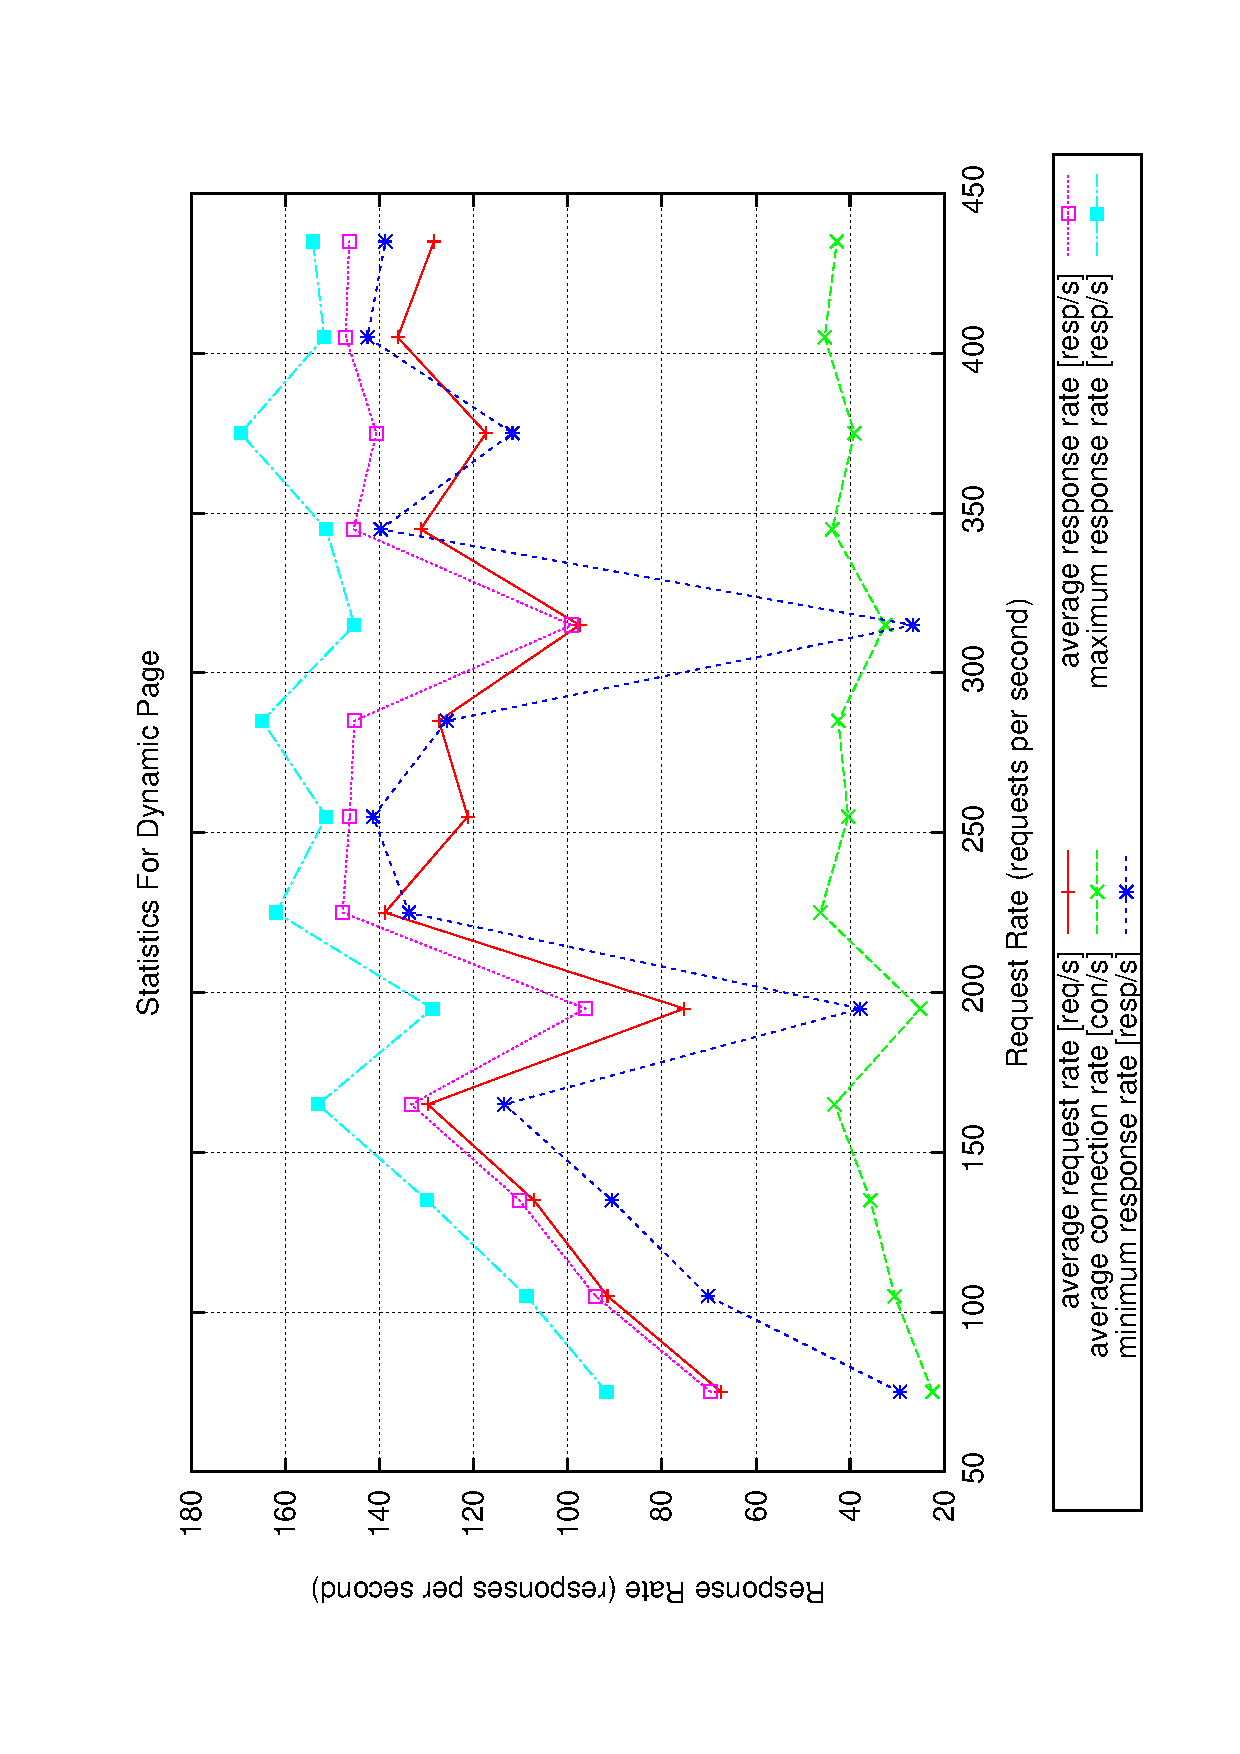
\includegraphics[scale=0.4]{charts/benchmarks/normal4.pdf}
  \end{center}
  \caption{Response rate statistics for dynamic page served using the Django framework.}
	\label{fig:sm_benchmark_normal}
\end{figure}
This number is close to the mentioned before short time limit of $7, 400$ requests per minute. The test were done several times that way to as close as possible to the this quota limits watching to receive replies with the \texttt{200 OK} response code. Additionally it is also interesting the observe the distribution of the minimum, average and maximum response rate with increasing value of average request rate. In ideal case all of this four factors would fallow identical linear curve.     

The second technique is cashing. It is a solution bundled into many web frameworks including Django which as noted  in Section~\ref{sec:gae_general} is supported by GAE. Concept of this technique is based on storing data in some fast accessible space called cache and with the help of it repeating calls can shorting the request path. A simple usage of cashing system could look as presented in Listing~\ref{code:py_cache}. The function \texttt{get\_from\_cache} returns the data calculated by function called \texttt{some\_time\_consuming\_calculations} that next becomes located into control of \texttt{memcache}\footnote{Memcached is a distributed, memory based cashing system. This only one of possible caching backends such like file-cache or database based storage engines however it is mostly used for its speed and support for multi-machine work mode.} for a time defined by the \texttt{expire\_time} variable. In case a subsequent calls coming before one hour from the first calculation of \texttt{data} they wont call the \texttt{some\_time\_consuming\_calculations} function but return the value stored by the \texttt{key} name.        
\lstset{language=Python,caption=Simple cache usage example in Python.,label=code:py_cache,
basicstyle=\scriptsize,         % the size of the fonts that are used for the code
showspaces=false,               % show spaces adding particular underscores
showstringspaces=false,         % underline spaces within strings
showtabs=false,                 % show tabs within strings adding particular underscores
tabsize=2,                    % sets default tabsize to 2 spaces
captionpos=b,                   % sets the caption-position to bottom
breaklines=true,                % sets automatic line breaking
breakatwhitespace=false,        % sets if automatic breaks should only happen at whitespace
escapeinside={\%*}{*)}          % if you want to add a comment within your code
}
\lstinputlisting{src/samples/py_cache.py}
When the \texttt{some\_time\_consuming\_calculations} is truly resource consuming this technique can bring efficient savings. In case test results for cached version of page the plot from Figure~\ref{fig:sm_benchmark_cache} does only slightly differ from the curves of the dynamic version from Figure~\ref{fig:sm_benchmark_normal}. Used HTTP headers shown in Listing~\ref{code:resp_headers} can help to avoid subsequent calls from a single user by using his browser-cache mechanisms.The test client was ignoring them as it was supposed to test the worst case scenario when all of the connections being opened come from different users that use browsers ignoring the cache specific headers including \texttt{Expires}, \texttt{Vary}, \texttt{Last\-Modified}, \texttt{ETag} and \texttt{Cache\-Control}. 
\lstset{language=HTML,caption=Server response headers for cached content.,label=code:resp_headers,
basicstyle=\scriptsize,         % the size of the fonts that are used for the code
showspaces=false,               % show spaces adding particular underscores
showstringspaces=false,         % underline spaces within strings
showtabs=false,                 % show tabs within strings adding particular underscores
tabsize=2,                    % sets default tabsize to 2 spaces
captionpos=b,                   % sets the caption-position to bottom
breaklines=true,                % sets automatic line breaking
breakatwhitespace=false,        % sets if automatic breaks should only happen at whitespace
escapeinside={\%*}{*)}          % if you want to add a comment within your code
}
\lstinputlisting{src/samples/headers_cache.txt}

On the other hand it does not mean that that using caching did not bring anything. Because the requests to cache are normally much cheaper from the requests that involve the server-side operations the binding quota limits are lower and allow for $8,640,000$ API calls a day. Usage of \texttt{memcached} did help to reduce the CPU usage what is a big advantage of this technique. However it should be taken into account that usage of memory caching will consume additional memory, make the system little more complex and by itself isn't a fault tolerant storage. Besides one of the biggest problems regarding cache is expiring it content. In case some page component changed on some of pages the easiest way is to flush all the cache content. In case of application that profile has similar number of read as write operations cache will be much harder to implement. This solution suits best applications of high read rate.      
\begin{figure}[ht]
  \begin{center}
	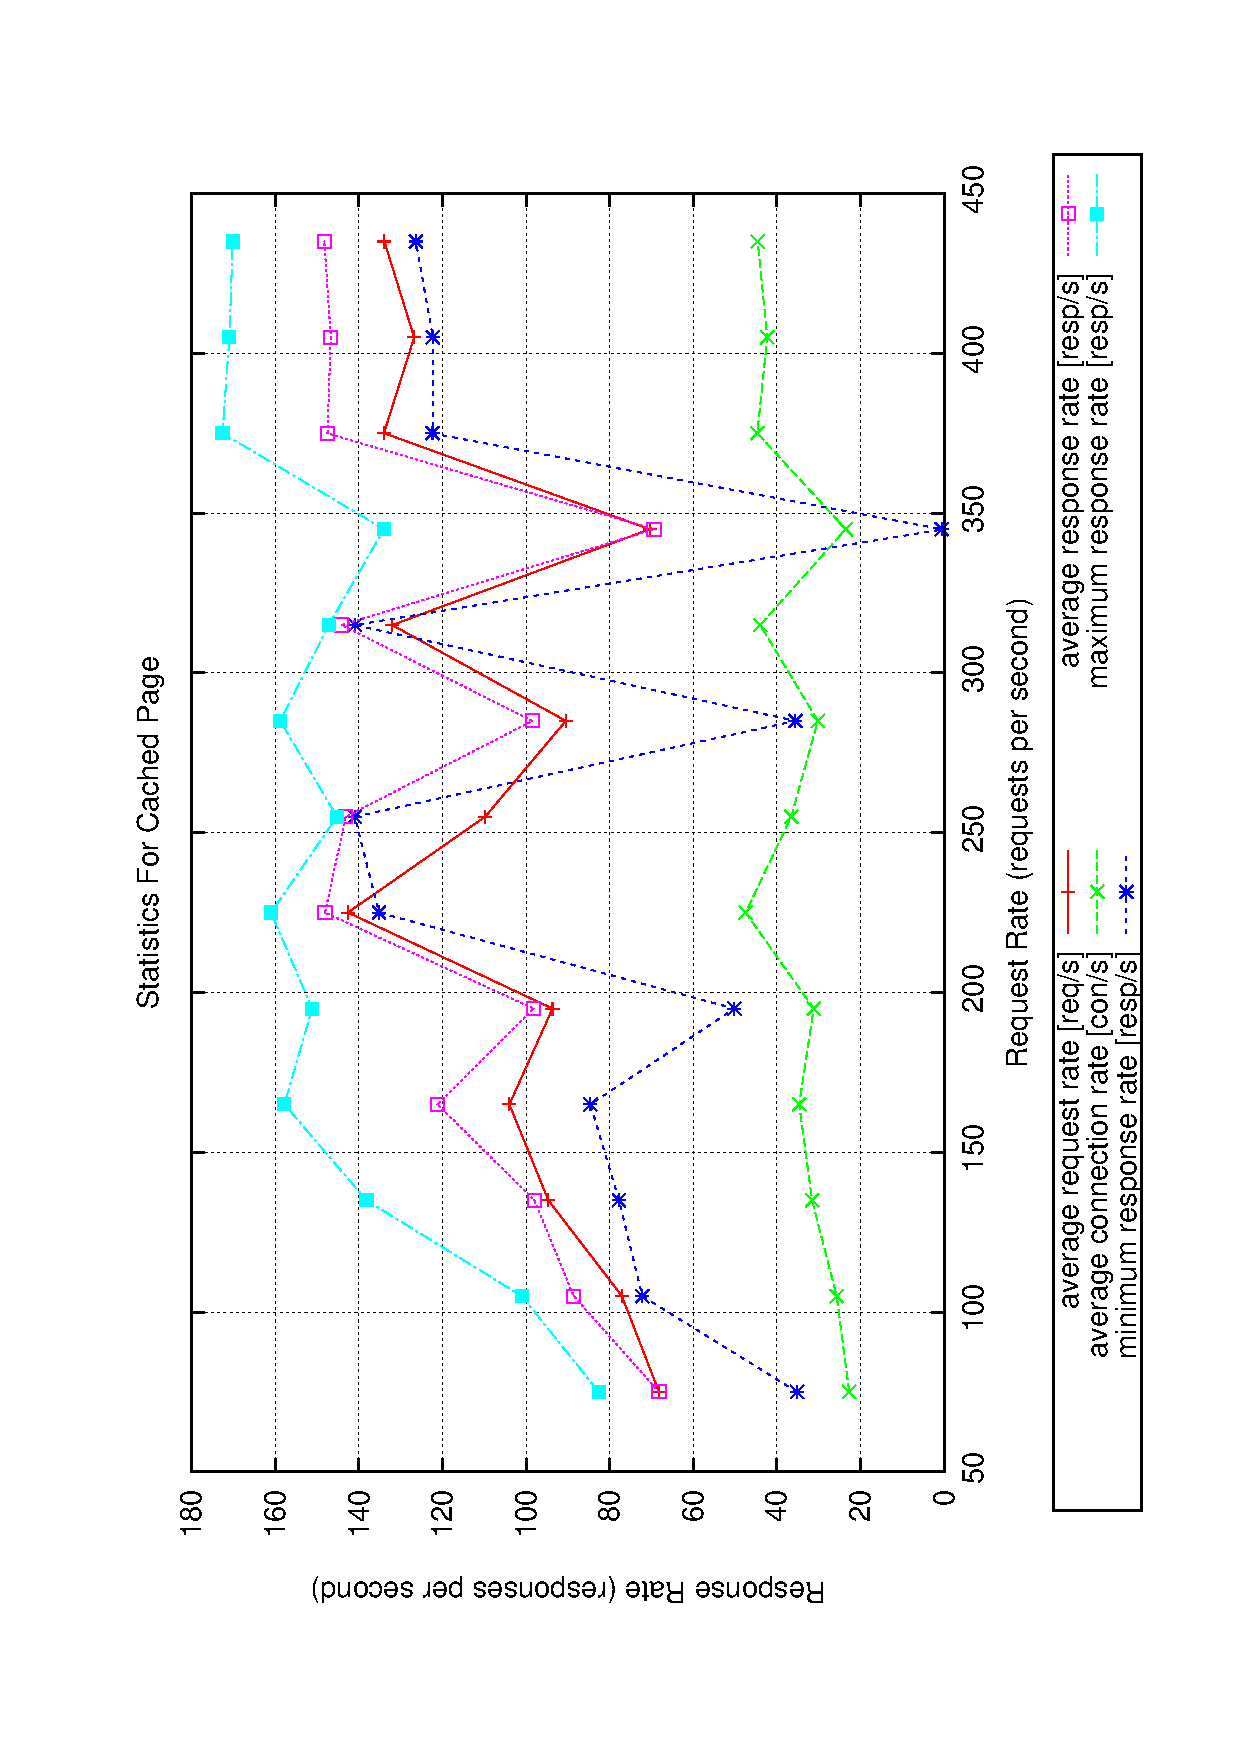
\includegraphics[scale=0.4]{charts/benchmarks/cache4.pdf}
  \end{center}
  \caption{Response rate statistics for cached page. Realised using the Google memcache API.}
  \label{fig:sm_benchmark_cache}
\end{figure}

The last tested approach was to serve the entire page as a static content. It should be noted that the infrastructure used for this purpose differs strongly from the application server. It takes the advantage of storing stateless content and minimum server overhead. The implementation details belong to the Google company however the they exist Open Source projects like \texttt{lighttpd} or \texttt{nginx} which share the same idea. Those differences can be easy observed in Figure~\ref{fig:sm_benchmark_static}. Until reaching the level of 235 requests per second the response rate curve was fallowing the server-side request rate curve with low value variation not crossing the factor of $5 \%$ of average value. In this case the CPU usage rate was even lower than using caching and did not require any additional memory usage like in case of \texttt{memcached}. It should be requires much more work to be integrated with the application replacing it prior dynamic content. That task might be sometimes even impossible to be done result in bed final experience when done not wright. Thus it definitely is interesting option for applications that are stateless or use lots of different media files.             
 \begin{figure}[ht]
  \begin{center}
	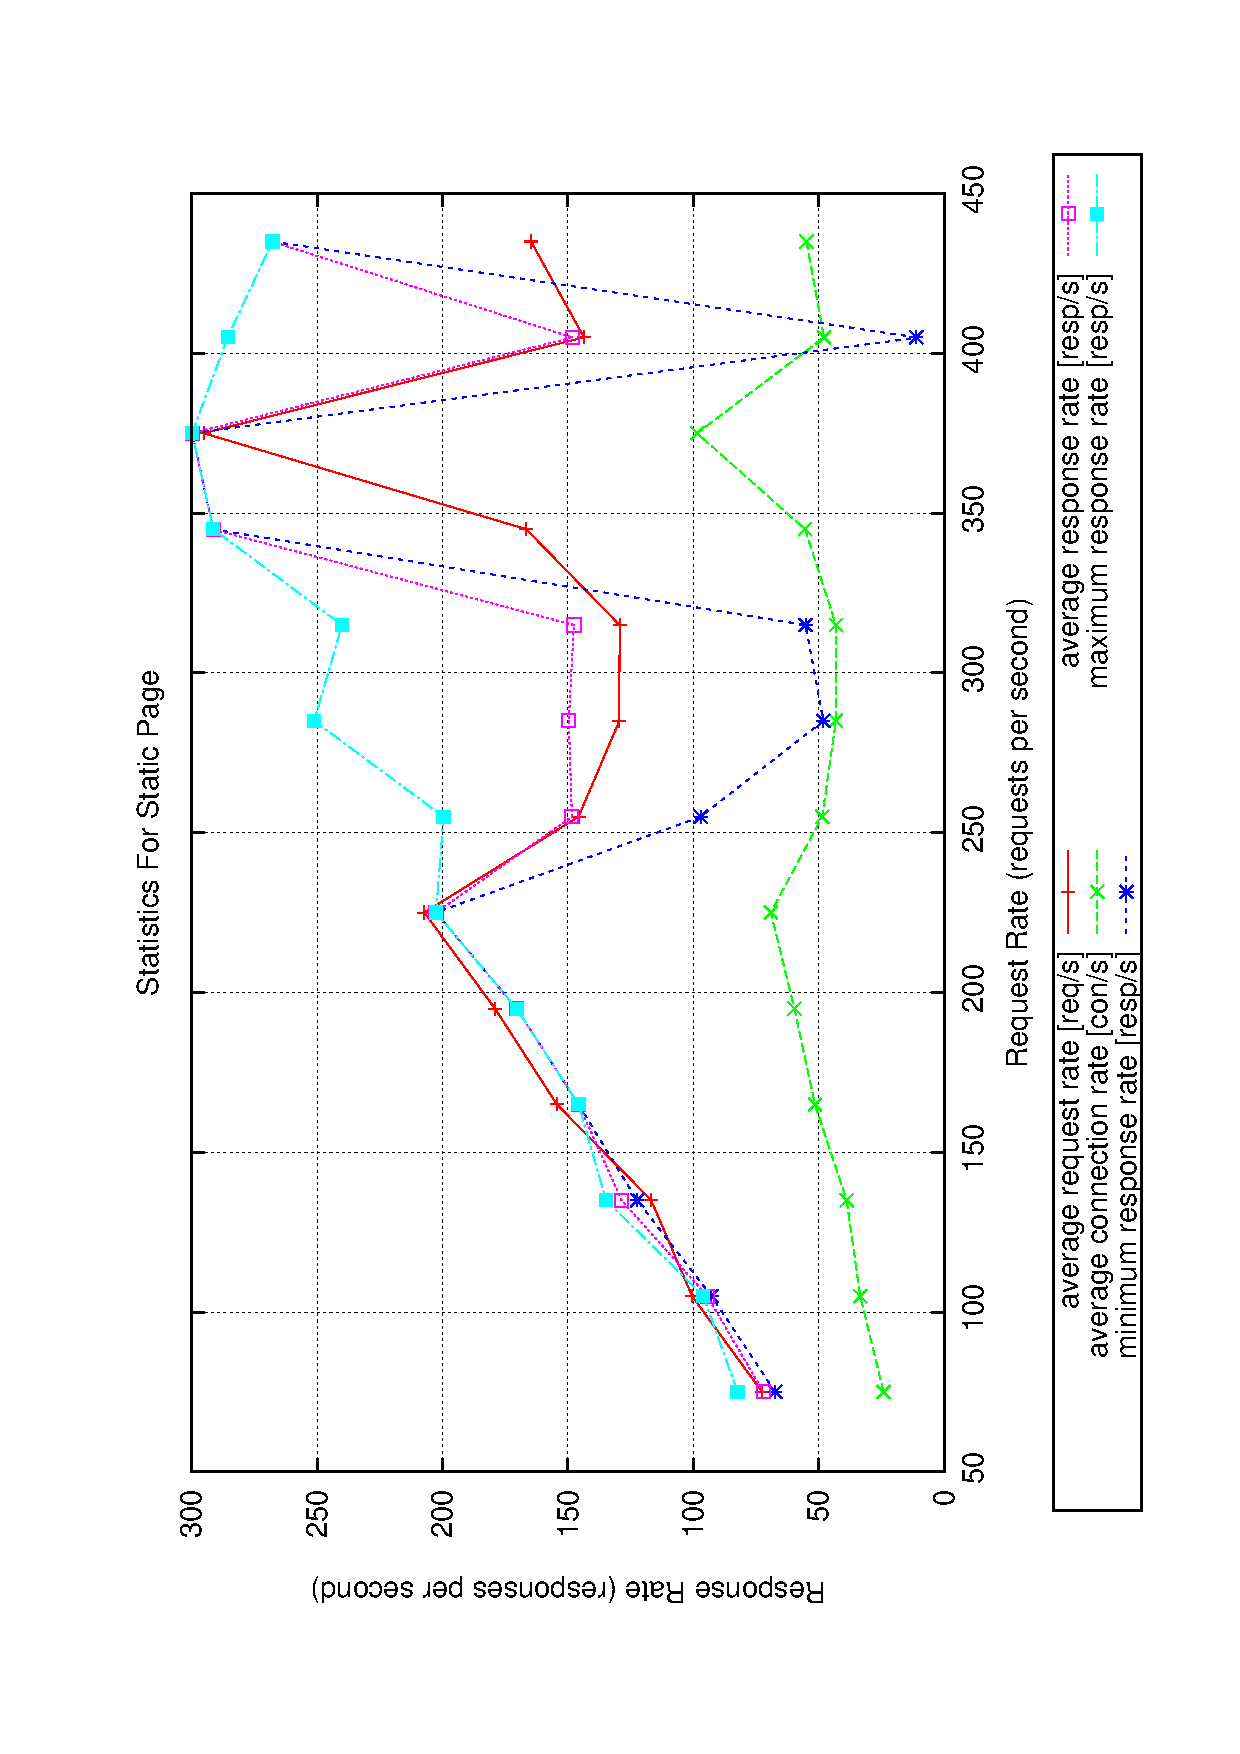
\includegraphics[scale=0.4]{charts/benchmarks/static4.pdf}
  \end{center}
  \caption{Response rate statistics for static page with use of static content server.}
\label{fig:sm_benchmark_static}
\end{figure}

An interesting comparison presented in Figure~\ref{fig:sm_resp_time_comapre} which collates various techniques used together by focusing on the average response time. It is one of the parameters that has a huge inpact on the user experience    
\begin{figure}[ht]
  \begin{center}
	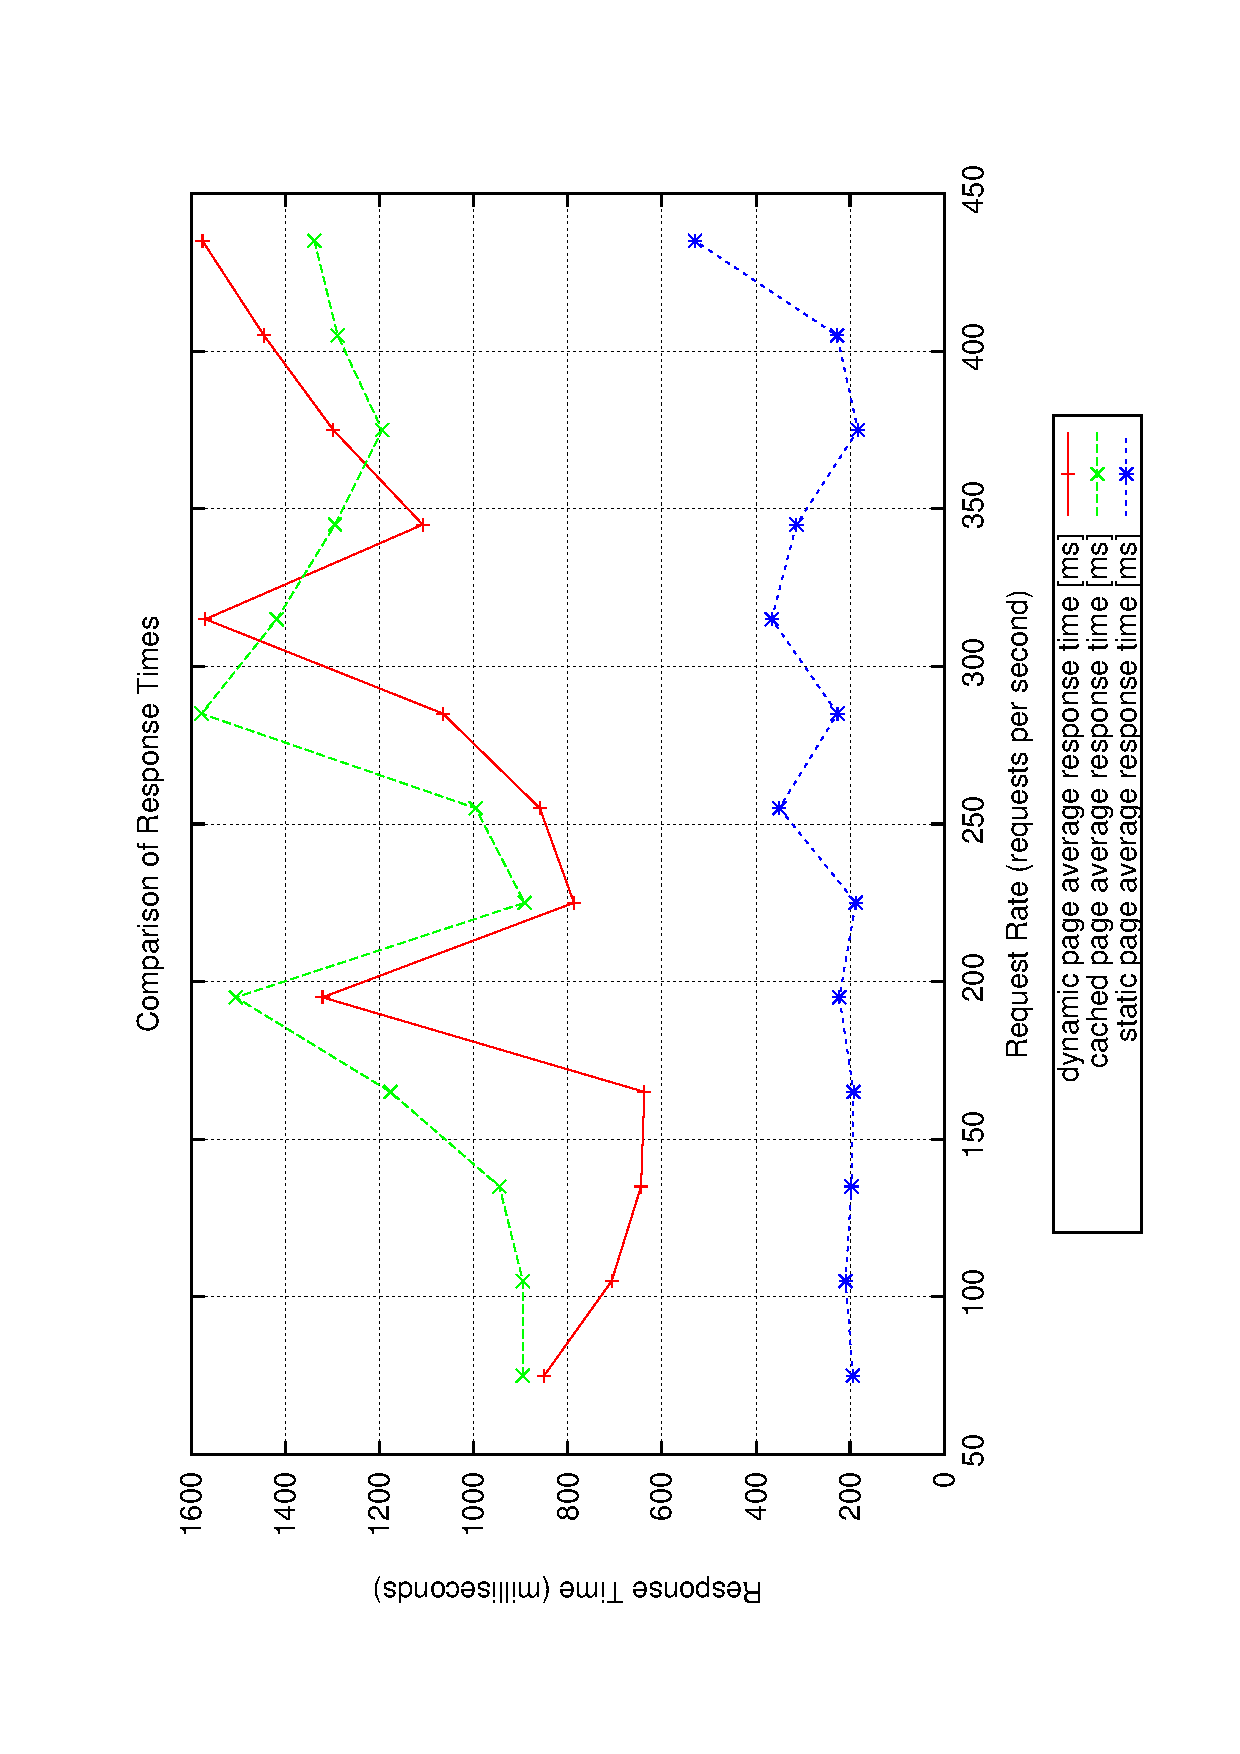
\includegraphics[scale=0.4]{charts/benchmarks/final4.pdf}
  \end{center}
  \caption{Comparison of average response times among various cases including serving dynamic content, caching response in memory or making use of static content server.}
	\label{fig:sm_resp_time_comapre}
\end{figure}  